\begin{abstract}
%----Image Teaser----%
\begin{figure}[!h]
    \begin{center}
        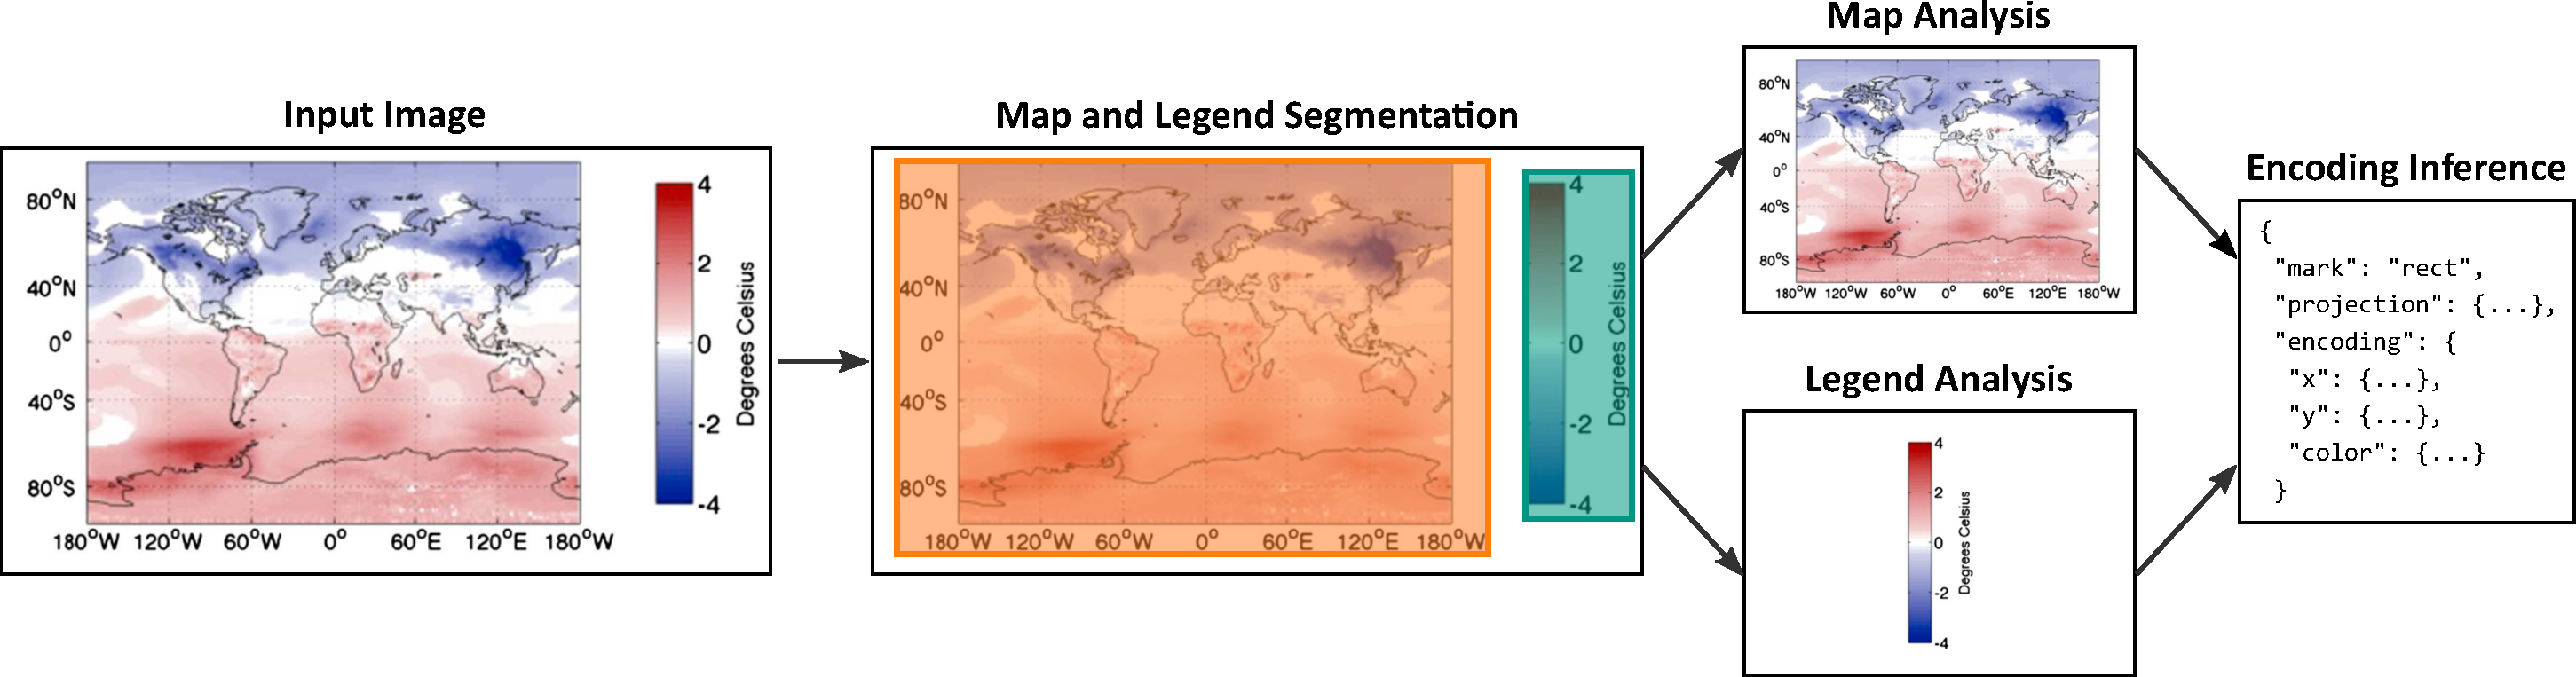
\includegraphics[width=\textwidth]{images/abstract_fig}
    \end{center}
\end{figure}

Map visualizations are used in diverse domains to show geographic data (\eg climate research, oceanography, business analyses, \etc).
These visualizations can be found in news articles, scientific papers, and on the Web.
However, many map visualizations are available only as bitmap images, hindering machine interpretation of the visualized data for indexing and reuse.

In this work, we propose a pipeline to recover the visual encodings from bitmap images of geographic maps with color-encoded scalar values.
We evaluate our results using map images from scientific documents, achieving high accuracy along each step of the pipeline.
In addition, we present iGeoMap, our web-based system that uses the extracted visual encoding to enable user-interaction over bitmap images of map visualizations.

\begin{flushleft}
\textbf{Keywords:} Visual encoding, Map interpretation, Map visualization.
\end{flushleft}

\end{abstract}
